\documentclass[a4paper, 11pt]{article}

\usepackage{customfonts}
\usepackage{pagelayout}
\usepackage{mathsettings}
\usepackage{computerscience}
\usepackage{float}
\let\emph\relax % there's no \RedeclareTextFontCommand
\DeclareTextFontCommand{\emph}{\bfseries}

\usepackage[mono,extrasp=0em]{inconsolata}


\usepackage{hyperref}
\hypersetup{
    colorlinks=true,
    linkcolor=green!50!black,
    filecolor=magenta,      
    urlcolor=blue!70!black,
    pdftitle={Assignment 1 DD2380},
    pdfpagemode=FullScreen,
    }
\urlstyle{same}

\setlength{\arrayrulewidth}{0.5mm}
\setlength{\tabcolsep}{18pt}
\renewcommand{\arraystretch}{1.5}

\title{Assignment 1 \\
DD2356}
\author{Johan Ericsson \quad joheric@kth.se}

\begin{document}
%\maketitle
%\begingroup  
%  \centering
%  \LARGE \sffamily Short Notes Template\\[1.0em]
%  \large Johan Ericsson \\ joheric@kth.se\par
%\endgroup

%\pretitle{\begin{center}\LARGE\color{RoyalBlue}}
%\posttitle{\par\end{center}\vskip 0.5em}

\maketitle

\textcolor{black}{\rule{\linewidth}{2pt}}
%{\sffamily
%This text describes the fundamental data structures commonly used.
%}
%
%\textcolor{black}{\rule{\linewidth}{2pt}}

\section{Sparse Matrix Vector Multiply}
We use the model
\[ T = nnz(2c + 2.5r) + n_r(0.5r + w), \]
for the execution time, $T$ of sparse matrix-vector multiply (SpMV). In our case there are five non-zero diagonals which leads to the
model
\[ T = 5 n_r(2c + 2.5r) + n_r(0.5r + w) = n_r(10c + 13r + w), \]
where $n_r$ denotes the number of rows, $c$, denotes the clock cycle, $r$ the time to read an element, and $w$ the time to write an element.
We use the simplified model
\begin{equation}\label{eq:time-sparse}
T = nnz 2c = 10cn_r.
\end{equation}
The processor we used for our measurements is an \textit{AMD Ryzen 5950X} processor which has a clock rate of 3.4 GHz (can be clocked up to 4.9),
which yields the clock cycle
\begin{equation}\label{eq:clock-cycle}
c = \frac{1}{3.4} \approx 0.294, \quad \text{(nanoseconds).}
\end{equation}



\subsection{Predicted execution times for SpMV}
By combining our model from equation (\ref{eq:time-sparse}) with the clock cycle calculated above in equation (\ref{eq:clock-cycle})
we are able to predict the expected execution times based on the matrix sizes. 

\begin{table}[H]\label{ta:predicted-times-sparse}
\centering
\begin{tabular}[c]{|c|c|}
\hline
number of rows $n_r$ &  estimated SpMV execution time (s) \\
\hline
$10^2$ & 2.941e-07 \\
$10^4$ & 2.941e-05 \\
$10^6$ & 0.002941 \\
$10^8$ & 0.2941 \\
\hline
\end{tabular}
\caption{Estimated execution times of SpMV on a 3.4GHz processor, using equation (\ref{eq:time-sparse}).}
\end{table}

\subsection{Measured execution times for SpMV}
Given the measured execution time, $T$ of the SpMV, and the number of rows, $n_r$,  we can estimate the floating-point operations per seconds
by the formula
\[ F = \frac{2nnz}{T} = \frac{10n_r}{T}, \quad \text{(flop/s).} \]

\begin{table}[H]\label{ta:measured-times-sparse}
\centering
\begin{tabular}[c]{|c|c|c|}
\hline
number of rows $n_r$ &  measured SpMV execution time (s) & Gflop/s \\
\hline
$10^2$ & 1e-6  & 1.0 \\
$10^4$ & 3.9e-5 & 2.564 \\
$10^6$ & 0.006261 & 1.597 \\
$10^8$ & 0.480609 & 2.081\\
\hline
\end{tabular}
\caption{Measured execution times of SpMV on a 3.4GHz \textit{AMD Ryzen 5950X} processor.}
\end{table}

\subsection{Predicted vs Measured execution times}

\subsection{Measured Read Bandwidths}

\subsection{STREAM Benchmark}
Below we display the STREAM benchmark output
\begin{lstlisting}[language=bash]
-------------------------------------------------------------
STREAM version $Revision: 5.10 $
-------------------------------------------------------------
This system uses 8 bytes per array element.
-------------------------------------------------------------
Array size = 10000000 (elements), Offset = 0 (elements)
Memory per array = 76.3 MiB (= 0.1 GiB).
Total memory required = 228.9 MiB (= 0.2 GiB).
Each kernel will be executed 10 times.
 The *best* time for each kernel (excluding the first iteration)
 will be used to compute the reported bandwidth.
-------------------------------------------------------------
Your clock granularity/precision appears to be 1 microseconds.
Each test below will take on the order of 6587 microseconds.
   (= 6587 clock ticks)
Increase the size of the arrays if this shows that
you are not getting at least 20 clock ticks per test.
-------------------------------------------------------------
WARNING -- The above is only a rough guideline.
For best results, please be sure you know the
precision of your system timer.
-------------------------------------------------------------
Function    Best Rate MB/s  Avg time     Min time     Max time
Copy:           19750.7     0.008989     0.008101     0.010046
Scale:          18208.4     0.010544     0.008787     0.011649
Add:            20437.6     0.012300     0.011743     0.012907
Triad:          20748.5     0.012294     0.011567     0.012824
-------------------------------------------------------------
Solution Validates: avg error less than 1.000000e-13 on all three arrays
-------------------------------------------------------------
 
\end{lstlisting}


\section{Memory Mountatin}
\subsection{Specifications of computer used for benchmarks}

The computer used for benchmarking has an \textit{AMD Ryzen 9 5950X} 16-core  processor with clock frequency 3.4GHz
The system is equipped with 32GiB (2x16 GiB) RAM and a 1TB SSD. The operating system is Ubuntu 20.04.4 LTS (linux kernel 5.13.0-39-generic).
The cache info is displayed in table \ref{table:cache-sizes} below.
\begin{table}[H]
\centering
\begin{tabular}{|c|c|}
 \hline
 Cache Level &  Cache size \\
 \hline
    L1d cache & 512 KiB \\
    L1i cache & 512 KiB \\
    L2 cache  & 8 MiB \\
    L3 cache  & 64 MiB \\
 \hline
\end{tabular}
\caption{\textit{AMD Ryzen 9 5950X} Cache sizes.}
\label{table:cache-sizes}
\end{table}


\subsection{Memory mountain}
The memory mountain ...
\begin{figure}[H]
\centering
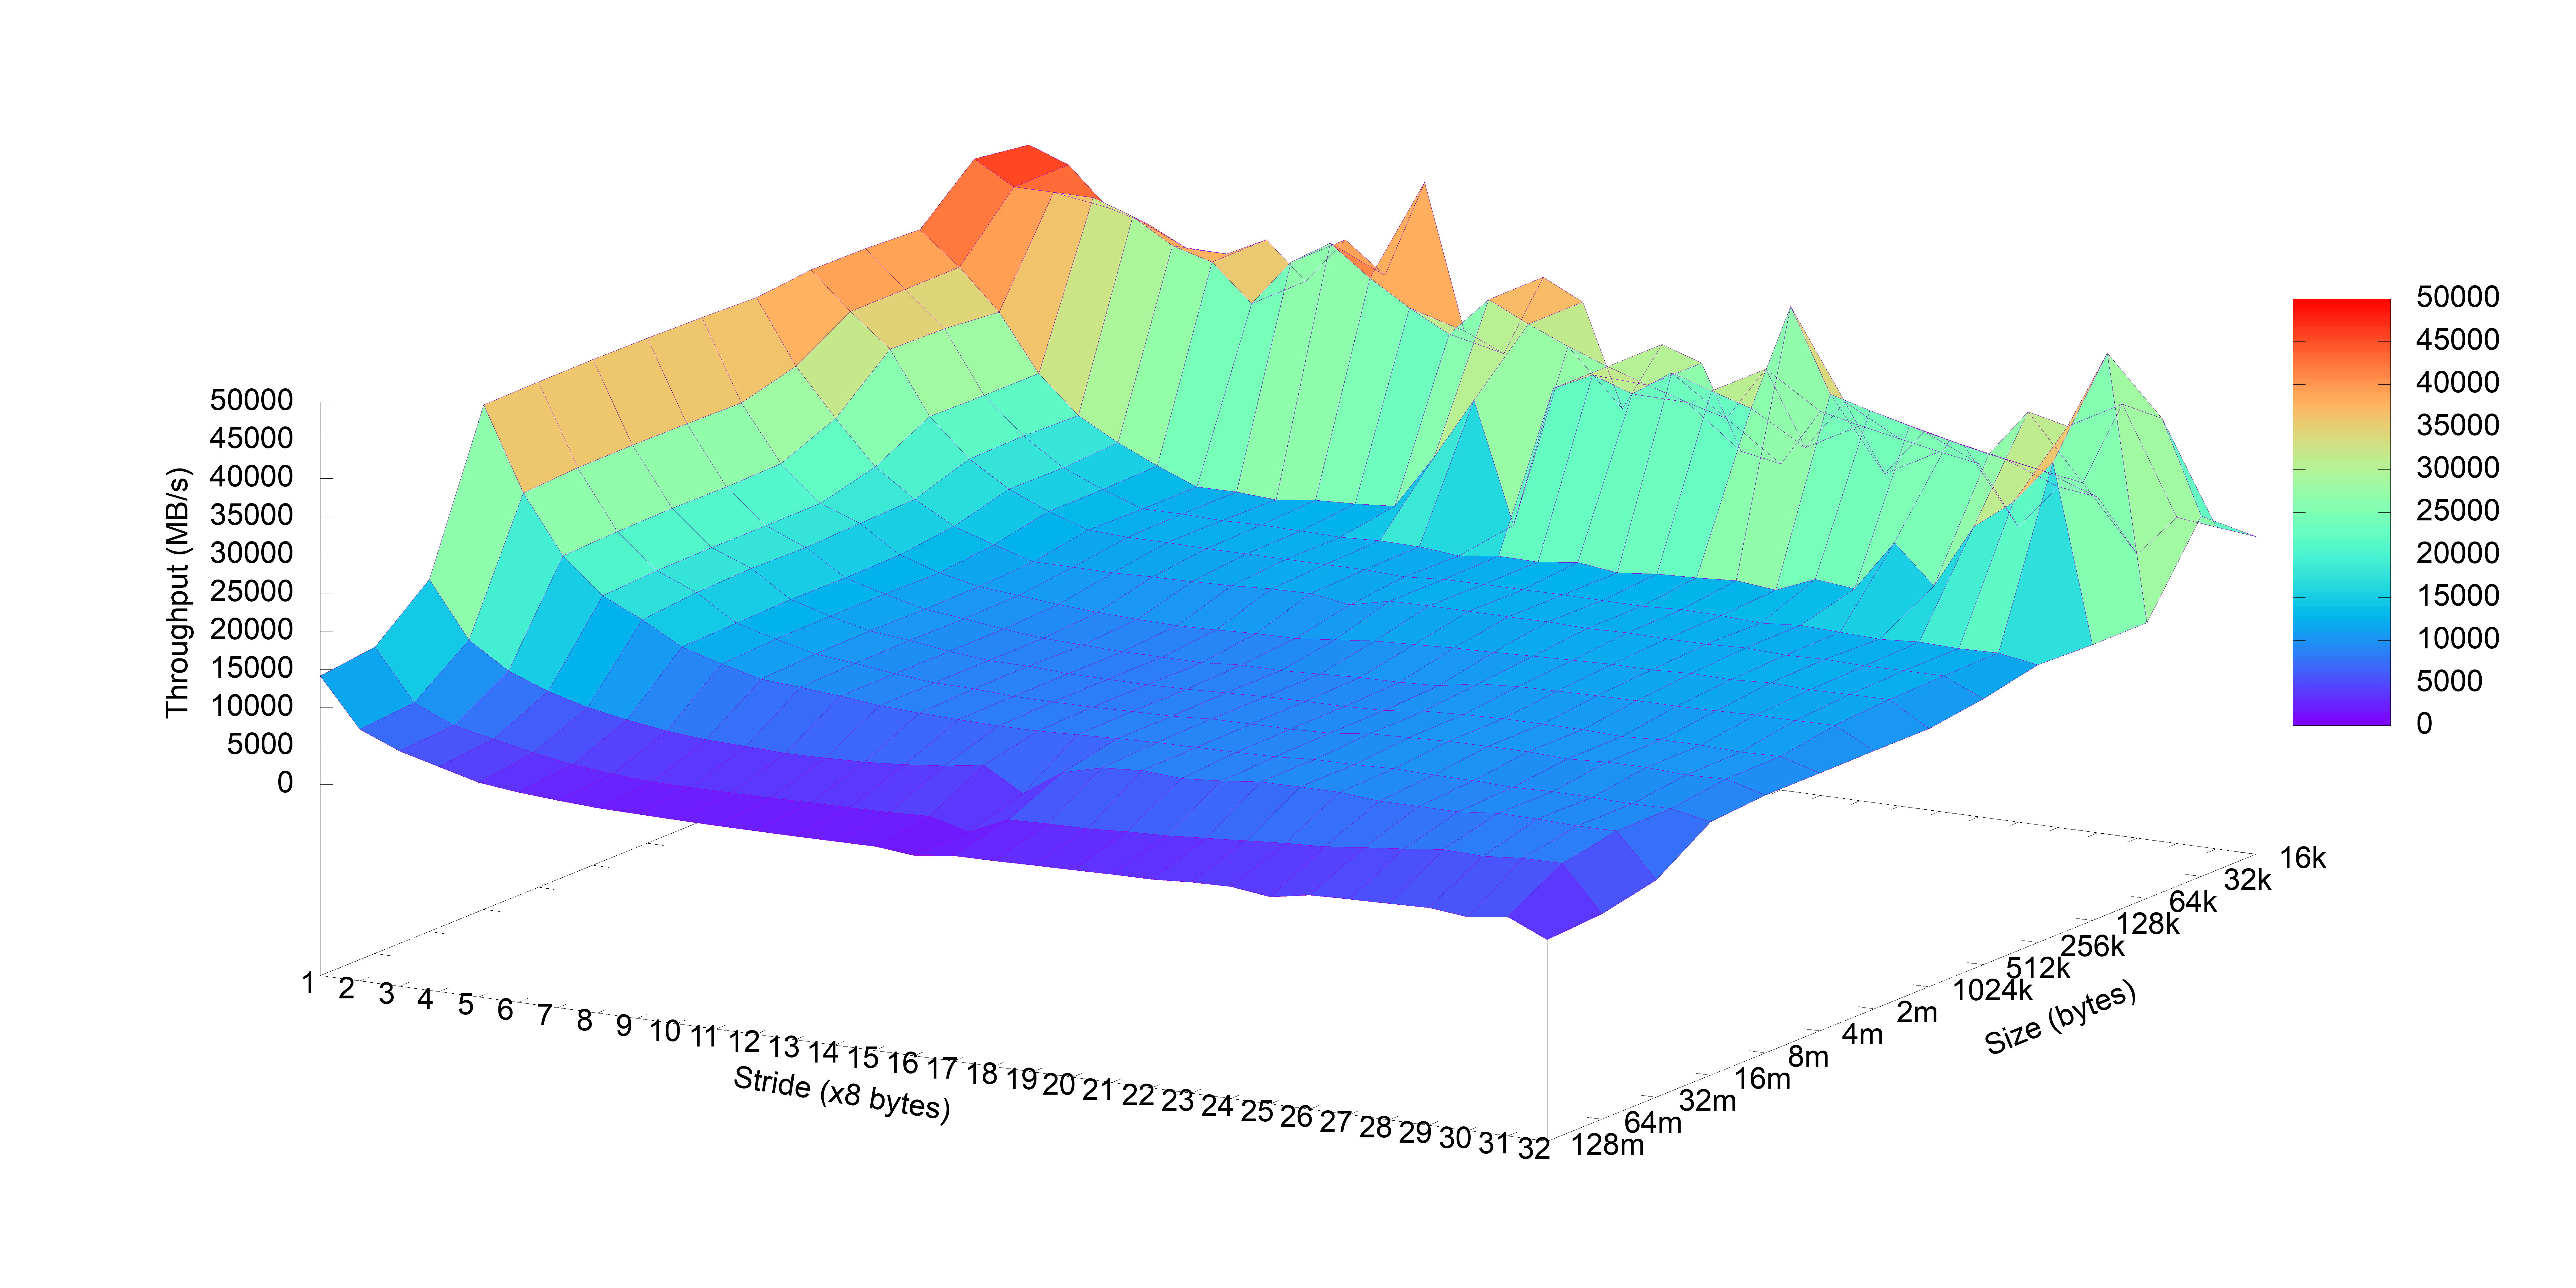
\includegraphics[width=\textwidth]{figures/memory_mountain.png}
\caption{Memory mountain.}
\end{figure}


\section{Writing Benchmark Code}
\subsection{Switching compiler environments on Dardel}
Compiler environments can be switched on Dardel using the \texttt{module swap} command. Switching from the cray compiler collection to the GNU collection
can be done with the command
\begin{lstlisting}
module swap PrgEnv-cray PrgEnv-gnu
\end{lstlisting}

\subsection{Average running time of \texttt{benchmark.c}}
The average running time of \texttt{benchmark.c} compiled with the GNU C compiler version 9.4.0 and optimization level 2 (-O2) was the same
when compiled with $N=5000$ and $N=10000$ at 0.00000095 (s).

\subsection{Analyzing the generated assembly}
The reason that the runtime remains unchanged with different sizes on the arrays is because of compiler optimizations. The compiler optimizes away the
code (the loop) between the timing measurements. This can be seen in listing \ref{listing:benchmark-asm-diff} which displays the relevant parts of the output
from the bash \texttt{diff} command applied to the optimized and unoptimized assembler generated from \texttt{benchmark.c}. This is clear when we run the code
compiled without optimizations, which for $N=10000$ had an average runtime of 0.00012207 (s).

\subsection{Clock Granularities}
\begin{lstlisting}
min dist = 9.54e-07, max dist = 1.19e-06, total time = 5.01e-06
\end{lstlisting}
Note the the clock granularity is the same as the measured the time with the optimized version which we ran by compiling \texttt{benchmark.c} with the -O2 flag.


\section{Cache Usage in Matrix-Matrix Multiply}

\begin{table}[H]\label{ta:measured-times-sparse}
\centering
\begin{tabular}[c]{|p{2cm}|p{2cm}|p{2cm}|p{2cm}|p{2cm}|}
\hline
event name & Naive \texttt{MSIZE=64} & Optimized \texttt{MSIZE=64} & Naive \texttt{MSIZE=1000} & Optimized \texttt{MSIZE=1000} \\
\hline
Elapsed time (s) &                  
Instructions per cycle
L1 cache miss ration &
L1 cache miss rate PTI &
LLC cache miss rate PTI &
\hline
\end{tabular}
\caption{Measured execution times of SpMV on a 3.4GHz \textit{AMD Ryzen 5950X} processor.}
\end{table}


\appendix
\section{Assembly output diff with/without optimizations}
\begin{lstlisting}[caption={Excerpt from the diff of the assembly generated for \texttt{benchmark.c} with optimization level -02 and with no optimization. Showing
lines which don't appear in the optimized version.},
label={listing:benchmark-asm-diff}]
> # benchmark.c:13:   for (i = 0; i < N; i++){
> 	movl	$0, -2400036(%rbp)	#, i
> # benchmark.c:13:   for (i = 0; i < N; i++){
> 	jmp	.L2	#
> .L3:
> # benchmark.c:14:     a[i] = 47.0;
> 	movl	-2400036(%rbp), %eax	# i, tmp89
> 	cltq
> 	movsd	.LC0(%rip), %xmm0	#, tmp90
> 	movsd	%xmm0, -2400016(%rbp,%rax,8)	# tmp90, a
> # benchmark.c:15:     b[i] = 3.1415;
> 	movl	-2400036(%rbp), %eax	# i, tmp92
> 	cltq
> 	movsd	.LC1(%rip), %xmm0	#, tmp93
> 	movsd	%xmm0, -1600016(%rbp,%rax,8)	# tmp93, b
> # benchmark.c:13:   for (i = 0; i < N; i++){
> 	addl	$1, -2400036(%rbp)	#, i
> .L2:
> # benchmark.c:13:   for (i = 0; i < N; i++){
> 	cmpl	$99999, -2400036(%rbp)	#, i
> 	jle	.L3	#,
> # benchmark.c:19:   t1 = mysecond();
> 	movl	$0, %eax	#,
> 	call	mysecond	#
> 	movq	%xmm0, %rax	#, tmp94
> 	movq	%rax, -2400032(%rbp)	# tmp94, t1
> # benchmark.c:20:   for(i = 0; i < N; i++)
> 	movl	$0, -2400036(%rbp)	#, i
> # benchmark.c:20:   for(i = 0; i < N; i++)
> 	jmp	.L4	#
> .L5:
> # benchmark.c:21:     c[i] = a[i]*b[i];
> 	movl	-2400036(%rbp), %eax	# i, tmp96
> 	cltq
> 	movsd	-2400016(%rbp,%rax,8), %xmm1	# a, _1
> # benchmark.c:21:     c[i] = a[i]*b[i];
> 	movl	-2400036(%rbp), %eax	# i, tmp98
> 	cltq
> 	movsd	-1600016(%rbp,%rax,8), %xmm0	# b, _2
> # benchmark.c:21:     c[i] = a[i]*b[i];
> 	mulsd	%xmm1, %xmm0	# _1, _3
> # benchmark.c:21:     c[i] = a[i]*b[i];
> 	movl	-2400036(%rbp), %eax	# i, tmp100
> 	cltq
> 	movsd	%xmm0, -800016(%rbp,%rax,8)	# _3, c
> # benchmark.c:20:   for(i = 0; i < N; i++)
> 	addl	$1, -2400036(%rbp)	#, i
> .L4:
> # benchmark.c:20:   for(i = 0; i < N; i++)
> 	cmpl	$99999, -2400036(%rbp)	#, i
> 	jle	.L5	#,
> # benchmark.c:22:   t2 = mysecond();
> 	movl	$0, %eax	#,
> 	call	mysecond	#
> 	movq	%xmm0, %rax	#, tmp101
> 	movq	%rax, -2400024(%rbp)	# tmp101, t2

\end{lstlisting}
\end{document}
